\documentclass[12pt]{article}

\usepackage{graphicx}
\usepackage{tikz}

\title{AMath Tea Time --- Puzzle \#6}
\author{}
\date{\vspace{-1cm}12 May 2015}

\begin{document}

\maketitle
\pagenumbering{gobble}

\subsection*{Problem}

\noindent {\it (This puzzle takes just a little bit of explaining...)} \\

\noindent A computer is constructed with a simple memory layout. It has an
unlimited amount of memory and each memory location is numbered so that a
program can refer to it. Each memory location can store a single number or be
uninitialized. In the following diagram the memory locations that are blank are
uninitialized and some other memory locations have numbers in them.

\begin{figure}[ht]
  \centering
  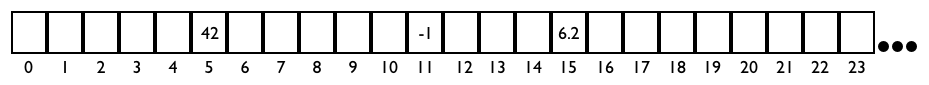
\includegraphics[width=\textwidth]{zmachine.png}
\end{figure}

\noindent The computer's CPU only has three instructions {\bf Z}, {\bf I} and
{\bf J} as follows:

\begin{itemize}
  \item[{\bf Z}] (Zero) This instruction zeroes a memory location. For example,
    {\bf Z}2 sets memory location 2 to 0 and {\bf Z}42 sets memory location 42
    to 0.
  \item[{\bf I}] (Increment) This instruction adds one to the contents of a
    memory location. For example, {\bf I}3 adds 1 to whatever is currently
    stored in location 3.
  \item[{\bf J}] (Jump) This instruction examines the contents of two memory
    locations and branches if the contents are different. For example {\bf
      J}18,19 would compare the contents of memory locations 18 and 19, if they
    are the same the program continues with the next instruction, if different
    it branches. The branch destination is just specified by drawing an arrow
    to the instruction you want to go to.
\end{itemize}

\noindent When there are no more instructions the program stops.

\pagebreak

\noindent For example, here's a loop that keeps adding one to memory location 4
until it equals memory location 20.

\begin{figure}[ht]
  \centering
  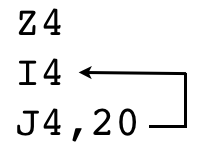
\includegraphics[width=100px]{zprogram.png}
\end{figure}

\noindent {\bf Question \#1:} The operator of the machine places two numbers
(one each) in memory locations 0 and 1. Here, for example, the operator has put
3 in location 0 and 4 in location 1. Write a program using the {\bf Z}, {\bf I}
and {\bf J} instructions to add those (arbitrary) numbers together and put the
result in memory location 2.

\begin{figure}[ht]
  \centering
  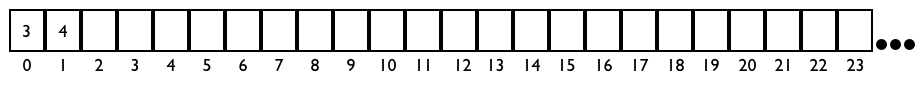
\includegraphics[width=\textwidth]{z34.png}
\end{figure}

\noindent {\bf Question \#2:} Under what circumstances does this program fail?


\subsection*{Hints}

{
\par\vspace*{\fill}
\noindent \small \it
If you have any puzzles to share then send them my way at {\tt
  cswiercz@uw.edu}!
}

\end{document}
